\documentclass[11pt]{article}

\usepackage[margin=1in]{geometry}
\usepackage{graphicx}
\usepackage{booktabs}
\usepackage{amsmath}
\usepackage{natbib}
\usepackage{hyperref}

\graphicspath{{figures/}}

\title{Partner-Specific Affective Precision Gates Social Policy Deployment in Multi-Agent Active Inference}
\author{TODO}
\date{Draft technical outline}

\begin{document}
\maketitle

\begin{abstract}
% One paragraph, not polished yet.
% Problem: active-inference accounts of affect often treat affective precision
% as a global action-model fitness signal.
% Gap: social interaction requires partner-specific model-fitness estimates.
% Method: repeated multi-partner trust game using official inferactively-pymdp
% agents plus an external HESP-style beta tracker per partner.
% Results: H1 30-seed confirmation shows precision tracks surprise more than
% reward; H2/H4 show deployment and social-choice movement in open regimes; H3
% shows abrupt betrayal can turn precision into misdeployment; gradual betrayal
% reduces the default affect penalty.
% Conclusion: affective precision is a partner-local deployment mechanism, not
% a generic reward booster.
\end{abstract}

\section{Introduction}

% Claim 1: Active inference explains action as policy inference under a
% generative model.
% Claim 2: Hesp-style affective precision can be read as model fitness over
% expected action precision.
% Claim 3: Social interaction creates a factorization problem: agents need to
% track model fitness separately for different partners.
% Claim 4: This paper tests whether partner-specific affective precision helps
% deploy social beliefs into action and partner choice.

Contributions to state explicitly:
\begin{enumerate}
  \item A partner-specific extension of affective precision in a repeated trust game.
  \item A supported implementation using official \texttt{inferactively-pymdp==1.0.0} for policy and state inference, with task-owned external beta tracking.
  \item Evidence that precision tracks prediction reliability more than reward.
  \item A boundary-condition result: abrupt betrayal can produce precision-driven misdeployment.
\end{enumerate}

\section{Model}

\subsection{Trust-game POMDP}

% Hidden factors: partner type, partner stance, own action.
% Observations: partner action and payoff.
% Controls: factorized stance and own-action controls inside each partner-local
% POMDP; partner choice is handled externally by evaluating partner-local agents.

The partner-local hidden state factors are:
\[
s = (s_{\mathrm{type}}, s_{\mathrm{stance}}, s_{\mathrm{own}})
\]
where type has four states, stance has three states, and own action is a
deterministic bookkeeping factor.

\subsection{External affective precision tracker}

% Beta is not a POMDP hidden state.
% Update signal is unsigned partner-action surprise: eps_k = 1 - P(observed action).
% Affective charge: phi_k = alpha (sigma_0^2 - eps_k^2).
% Mapping to policy precision: gamma_k = gamma_base / E[beta_k].
% Lesion: beta updates continue but gamma is fixed at baseline.

\begin{equation}
\epsilon_k = 1 - P(o^{\mathrm{action}}_k \mid q(s_{\mathrm{type}}, s_{\mathrm{stance}}))
\end{equation}

\begin{equation}
\phi_k = \alpha(\sigma_0^2 - \epsilon_k^2)
\end{equation}

\begin{equation}
\gamma_k = \gamma_{\mathrm{base}} / \mathbb{E}[\beta_k]
\end{equation}

\begin{figure}[t]
  \centering
  % TODO: replace with final schematic.
  \fbox{\parbox{0.85\linewidth}{Model schematic placeholder: partner prediction error $\rightarrow$ beta/precision $\rightarrow$ partner-local gamma $\rightarrow$ policy posterior $\rightarrow$ deployment.}}
  \caption{Partner-specific affective precision architecture. Each partner has a local \texttt{pymdp.Agent}; beta is an external HESP-style tracker that modulates partner-local policy precision.}
  \label{fig:model-schematic}
\end{figure}

\section{Experiments}

% Use behavior-card structure H0-H5.
% Emphasize that payoff is downstream; primary readouts include entropy,
% precision-surprise association, belief accuracy, selection rates, and
% misdeployment rates.

\begin{table}[t]
  \centering
  \caption{Manuscript evidence hierarchy.}
  \label{tab:evidence-hierarchy}
  \begin{tabular}{llll}
    \toprule
    Card & Primary role & Seeds & Manuscript status \\
    \midrule
    H0 & Openness gate & 5/variant & Supporting \\
    H1 & Model fitness & 30/variant & Primary \\
    H2 & Deployment dissociation & 5/variant & Supporting \\
    H3 & Stress boundary & 30/variant & Primary \\
    H4 & Social choice & 5/variant & Supporting \\
    H5 & Perturbation dynamics & 5/variant & Supplemental \\
    \bottomrule
  \end{tabular}
\end{table}

\section{Results}

\subsection{Open policy spaces permit affective deployment}

% H0/H2, five seeds.
% Affect payoff 1884.6 vs no-affect/lesion 1859.4.
% Entropy 7.94 vs 8.80.
% State as supporting evidence because n=5 per variant.

\begin{figure}[t]
  \centering
  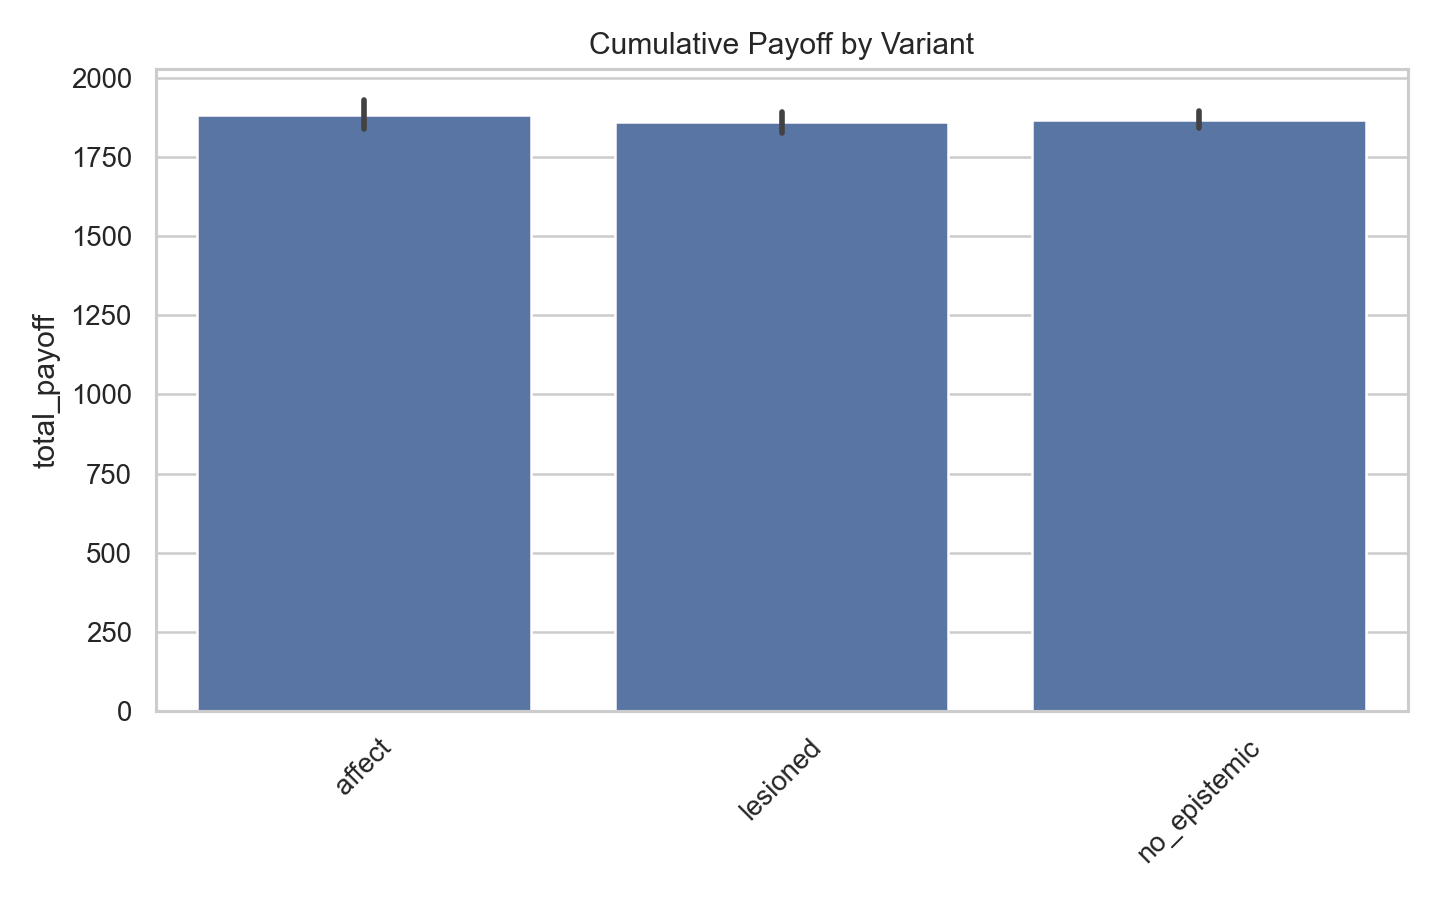
\includegraphics[width=0.8\linewidth]{fig_open_regime_cumulative_payoff.png}
  \caption{Open-regime deployment. In the graded open-policy regime, affect lowers policy entropy and improves payoff relative to the lesioned/no-affect baseline, while belief readouts remain similar.}
  \label{fig:open-regime}
\end{figure}

\subsection{Partner-specific precision tracks model fitness rather than reward}

% H1 confirmation, 30 seeds per variant.
% Total payoff affect 534.6 vs no-affect 542.1; no payoff advantage.
% |corr(precision, surprise)| = 0.701 vs |corr(precision, payoff)| = 0.419.
% Reliability-over-reward effect +0.096, CI [0.027, 0.164].

\begin{figure}[t]
  \centering
  
\includegraphics[width=0.8\linewidth]{fig_model_fitness_beta_reward_divergence.png}
  \caption{Model-fitness readout. Partner-specific precision tracks predictive surprise more strongly than realized payoff in the 30-seed H1 confirmation.}
  \label{fig:model-fitness}
\end{figure}

\subsection{Affect changes deployment despite similar belief accuracy}

% H2, five seeds.
% Affect: payoff 1884.6, joint accuracy 0.336, stance accuracy 0.816, entropy 7.94.
% Lesion: payoff 1859.4, joint accuracy 0.339, stance accuracy 0.855, entropy 8.80.
% Framing: knowing-versus-using, not vmPFC implementation.

\subsection{Partner choice changes before payoff}

% H4, five seeds.
% Payoff flat: 393.6 vs 393.2.
% Entropy changes: 3.99 vs 4.83.
% Selection rates: affect [0.366, 0.316, 0.138, 0.180];
% no-affect [0.348, 0.318, 0.162, 0.172].

\subsection{Abrupt betrayal exposes a precision-driven boundary condition}

% H3 confirmation, 30 seeds per variant.
% Affect payoff 1136.1 vs no-affect/lesion 1172.1, p=0.0169.
% Entropy 8.38 vs 8.74.
% Reencounters 4.4 vs 6.1; selection rate 0.049 vs 0.067.
% Payoff on reencounter 8.76 vs 8.91.
% Wrong-type rate 0.237 vs 0.165.
% Claim: active but not safer; do not claim recovery win.

\begin{figure}[t]
  \centering
  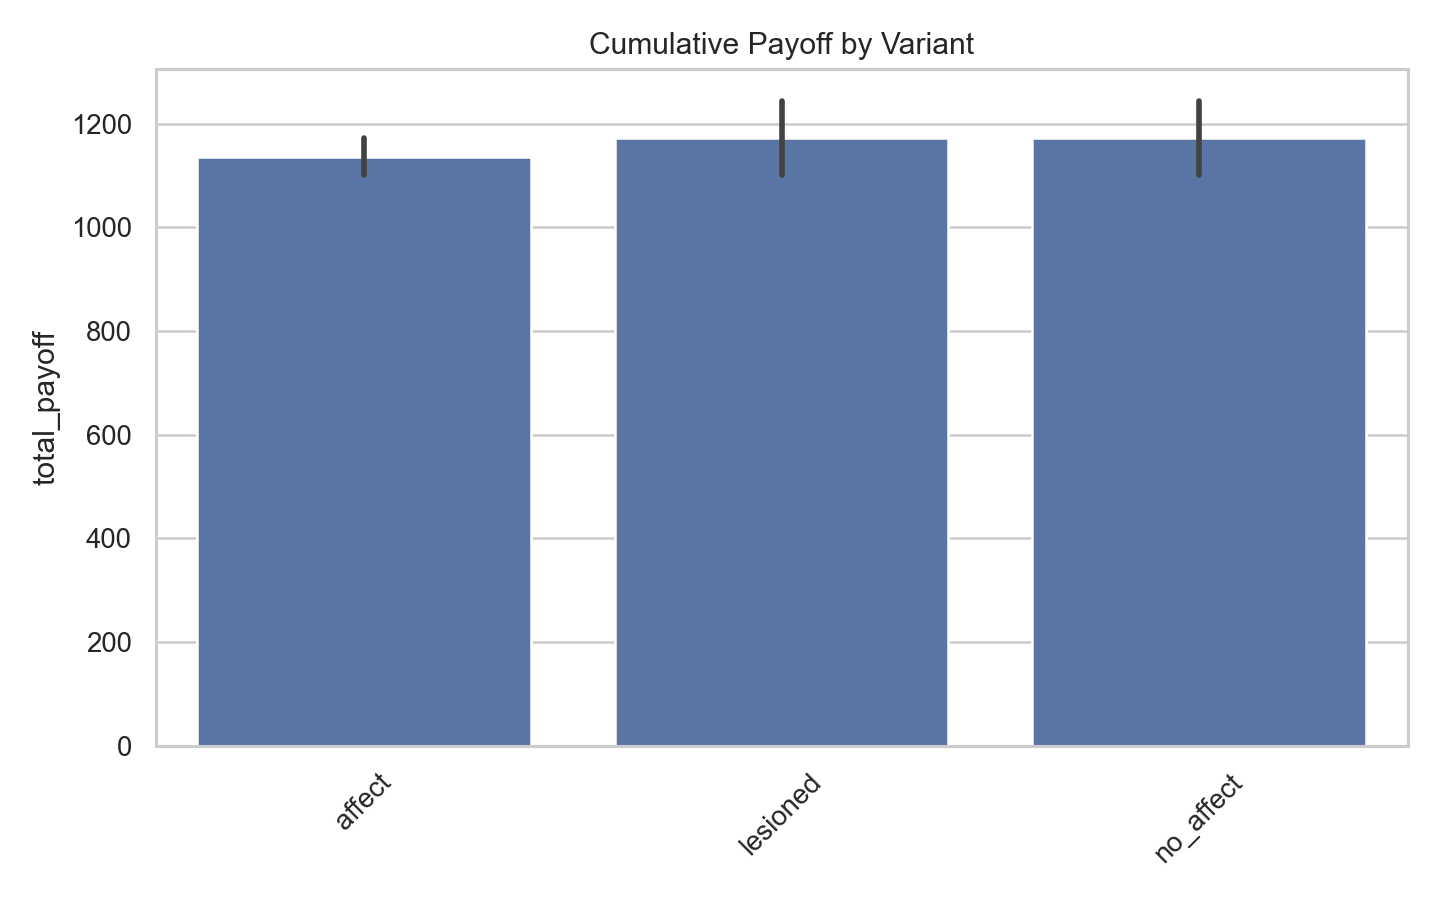
\includegraphics[width=0.48\linewidth]{fig_betrayal_confirm_cumulative_payoff.png}
  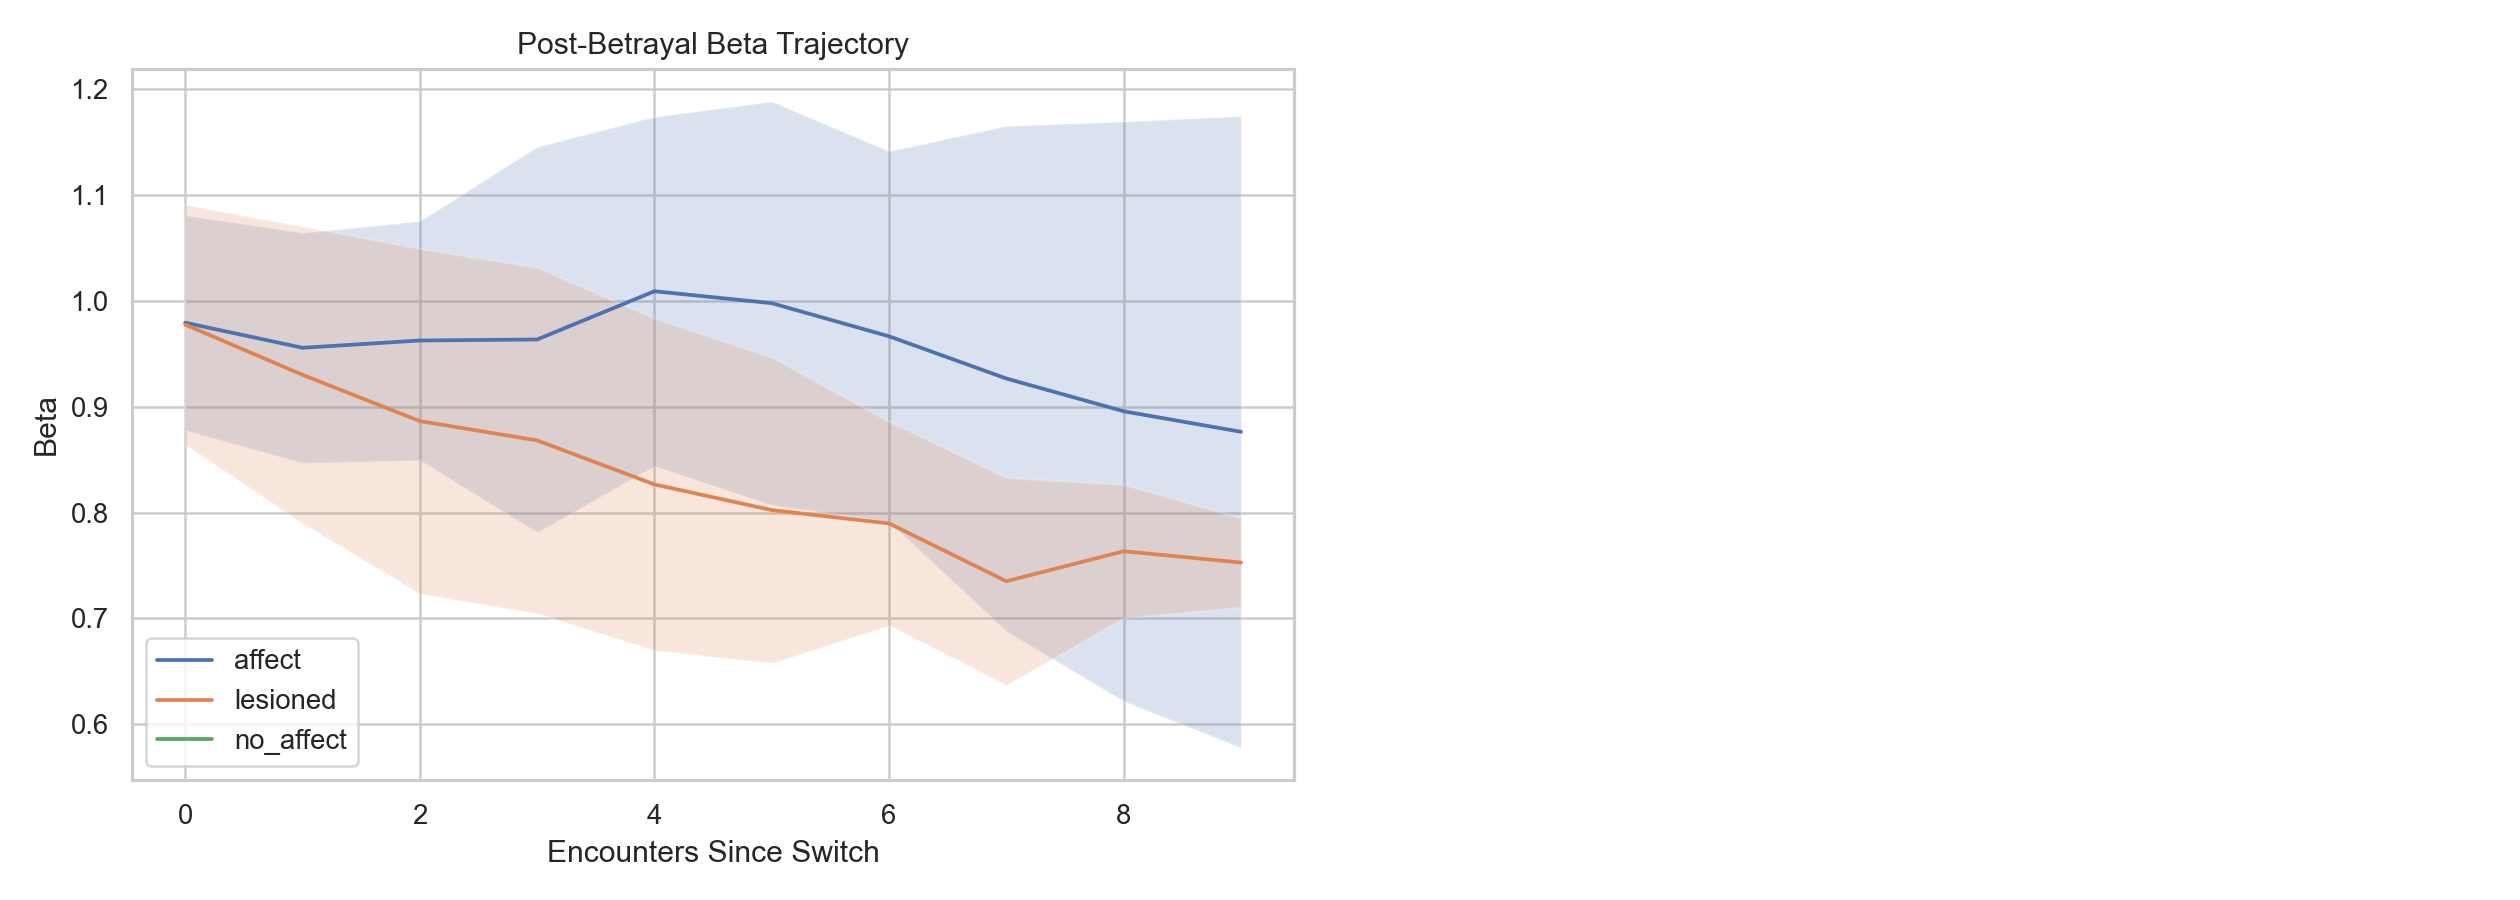
\includegraphics[width=0.48\linewidth]{fig_betrayal_signal_trajectories.png}
  \caption{Betrayal boundary condition. Affective precision lowers entropy and changes reallocation after an abrupt stance switch, but whole-run payoff and conditional return payoff do not improve.}
  \label{fig:betrayal-boundary}
\end{figure}

\subsection{Shock shape matters more than generic caution}

% H3 sensitivity, 30 seeds per variant.
% Abrupt no-affect/lesion 1153.6; default affect 1140.4, p=0.370; combined
% caution 1115.0, p=0.003.
% Gradual no-affect/lesion 1148.9; default affect 1147.6, p=0.906; combined
% caution 1118.3, p=0.005.
% Claim: generic caution is not the repair; abruptness is the important axis.

\begin{figure}[t]
  \centering
  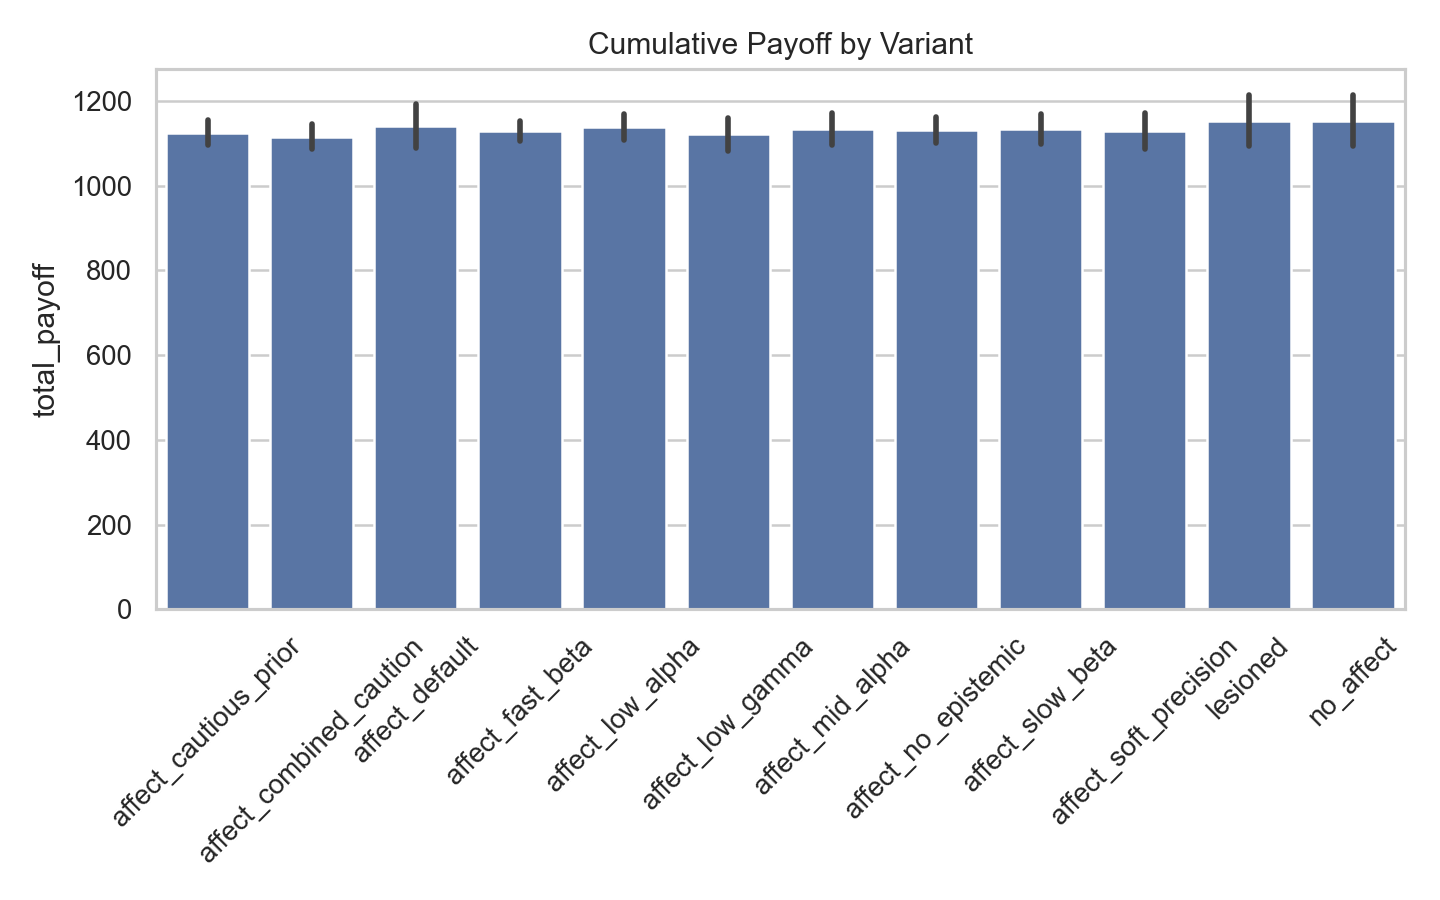
\includegraphics[width=0.48\linewidth]{fig_abrupt_sensitivity_cumulative_payoff.png}
  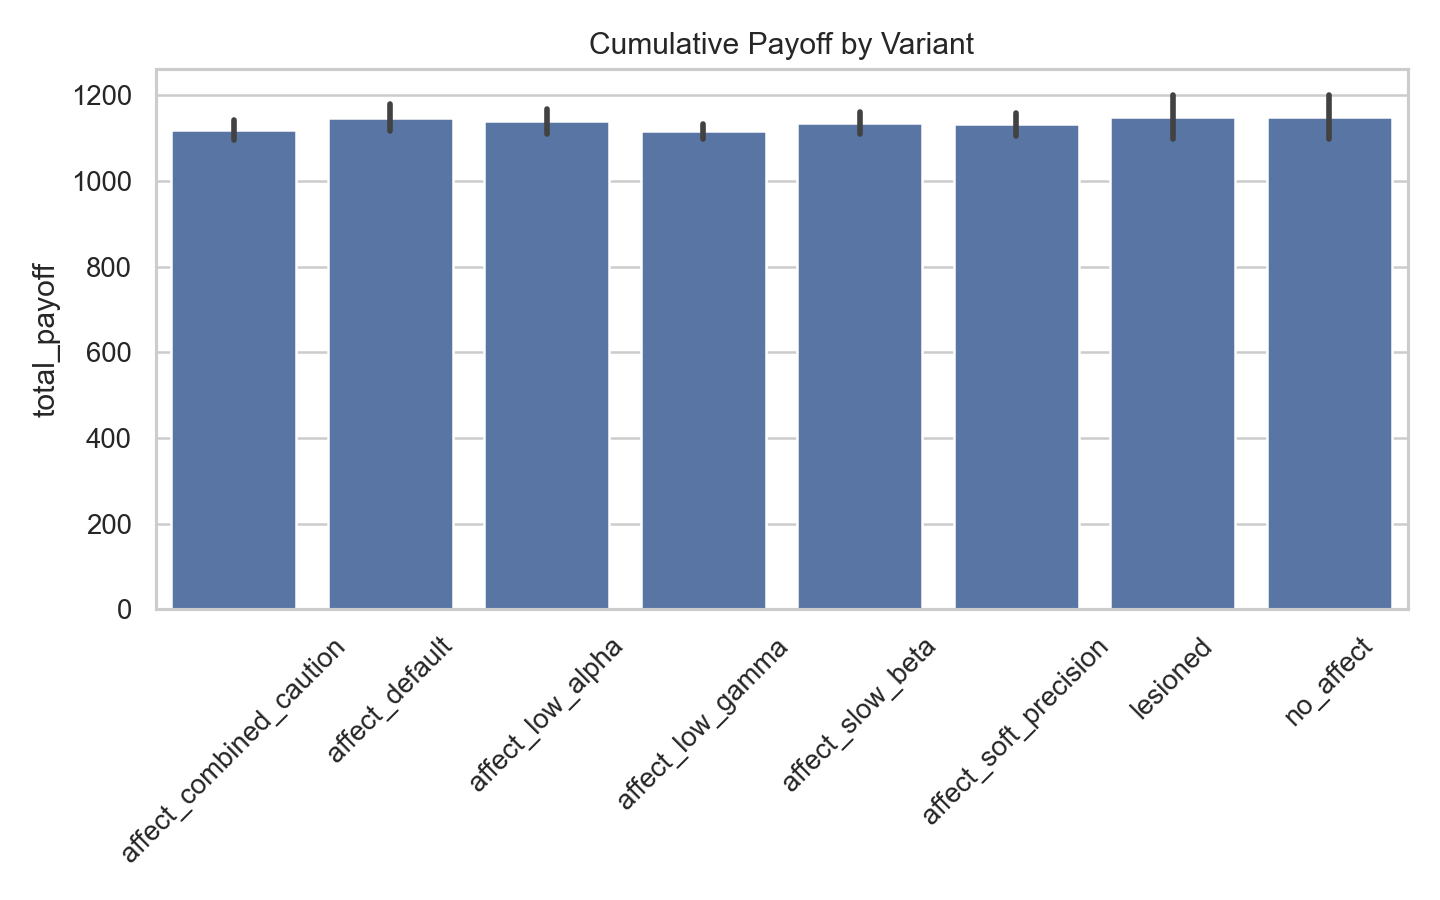
\includegraphics[width=0.48\linewidth]{fig_gradual_sensitivity_cumulative_payoff.png}
  \caption{Shock-shape sensitivity. Default affect is costly under abrupt betrayal but nearly payoff-neutral under gradual betrayal; generic caution variants raise entropy without rescuing payoff.}
  \label{fig:shock-shape}
\end{figure}

\subsection{Clinical-like perturbations separate precision dynamics}

% Supplemental H5, five seeds.
% Dynamics beta range: borderline 1.318, depression 1.435, affect 0.950,
% alexithymia 0.149.
% Betrayal payoff: alexithymia 1216.3, borderline 1196.9, affect 1168.3,
% depression 1150.1.
% Must say clinical-like parameter perturbations, not clinical validation.

\section{Discussion}

Main interpretation:
\begin{itemize}
  \item Partner-local affective precision is computational infrastructure for deploying social beliefs.
  \item Precision tracks model fitness, not reward or partner liking.
  \item Policy openness is necessary for visible behavioral effects.
  \item Abrupt social shocks can misalign belief recalibration and policy sharpening.
\end{itemize}

Alternatives to rule out or bound:
\begin{itemize}
  \item Not a global payoff-improvement result.
  \item Not a literal trust scalar.
  \item Not just deeper planning; planning horizon is a controlled variant knob.
  \item Not a clinical model.
\end{itemize}

\section{Limitations}

\begin{itemize}
  \item Simulation-only evidence.
  \item Scripted partner behavior in the primary trust task.
  \item H0/H2/H4 and H5 are five-seed supporting results.
  \item No global-beta ablation yet, so partner specificity is not directly compared to global affect.
  \item H5 perturbations are clinical-like parameter changes, not validated clinical phenotypes.
  \item Current figures are analysis diagnostics and should be redrawn for submission.
\end{itemize}

\section{Future Work}

Priority before deadline:
\begin{enumerate}
  \item Create final composite figures from current source tables.
  \item If implementation time allows, run a global-beta ablation.
  \item If experiment time allows, run a focused shock-shape gradient rather than a broad hyperparameter sweep.
\end{enumerate}

\section{Conclusion}

% Final claim: partner-specific affective precision plausibly bridges social
% model fitness and policy deployment. The current evidence supports the
% mechanism and its boundary condition while leaving human validation,
% global-beta comparison, and broader model comparison for future work.

\bibliographystyle{apalike}
\bibliography{references}

\end{document}
